\documentclass{beamer}
%\usetheme{Warsaw}
\usetheme{MAUA}


\usepackage[utf8]{inputenc}
\usepackage[T1]{fontenc}
\usepackage{minted}

\usepackage[brazil,brazilian]{babel}
\usepackage{graphicx}
\graphicspath{./Figs/}
\usepackage{todonotes}

%==========================================================================
\title{Desenvolvimento de Mancal Magnético  para Rodas de Reação}
\subtitle{Qualificação Mestrado}
\author{Rafael Corsi Ferrão}
\date{\today}
\institute{\url{rafael.corsi@maua.br} \\\url{http://www.maua.br}}
%==========================================================================

\newcommand{\executeiffilenewer}[3]{%
\ifnum\pdfstrcmp{\pdffilemoddate{#1}}%
{\pdffilemoddate{#2}}>0%
{\immediate\write18{#3}}\fi%
}

\newcommand{\includesvg}[1]{%
\executeiffilenewer{#1.svg}{#1.pdf}%
{inkscape -z -D --file=./Figs/#1.svg %
--export-pdf=./Figs/#1.pdf --export-latex}%
\input{./Figs/#1.pdf_tex}%
}


\begin{document}

\begin{frame}[plain,t]
	\titlepage
\end{frame}

\begin{frame}
	\frametitle{Conteúdo}
		\tableofcontents
\end{frame}
%==========================================================================

\section{Introdução}

\subsection{Rodas de Reação}
\begin{frame}{Rodas De Reação}

	\begin{itemize}
		\item atuador eletromecânico
		\item conservação de momento angular
		
	 	%$h_{total} = I_{s} \frac{d \theta_{s}}{d t} + I_{r} \frac{d \theta_{r}}{d t}$
	\end{itemize}
	
	\begin{center}
	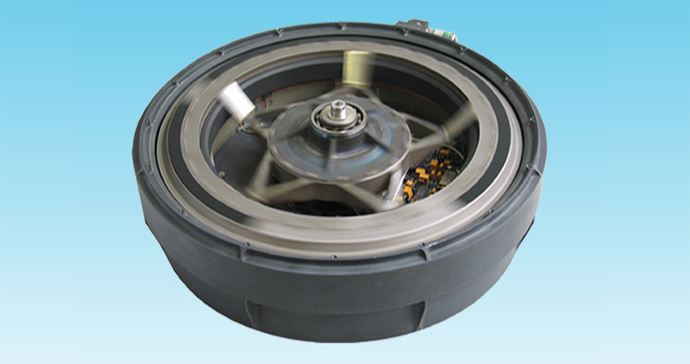
\includegraphics[width=0.5\linewidth]{MWI.jpg}
	\end{center}
	
	é constituída de :
	
	\begin{itemize}
		\item Motor de corrente contínua sem escovas (BLDC)
		\item Inércia
		\item Mancal
		\item Eletrônica
	\end{itemize}
\end{frame}

\begin{frame}{Mancal mecânico}
	
	Solução mais usual porém apesar de sua aparente simplicidade apresenta sérios desafios:

	\begin{itemize}
		\item Lubrificantes (Ciclos térmicos, radiação, pressão atmosférica)	
		\begin{itemize}
			\item Fluida
			\item Seca
		\end{itemize}
		\item Eventual necessidade de um selamento hermético 
		\item Difícil modelagem
	\end{itemize}
	
\end{frame}

\begin{frame}{Solução proposta}

	Mancal magnético:

	\begin{itemize}
		\item solução sem contato mecânico entre o estator e rotor
		\item confiabilidade depende basicamente da eletrônica
		\item validação em ambiente terrestre 
		\item eliminação da zona morta
		\item aumento na complexidade da malha de controle
	\end{itemize}
\end{frame}

%\begin{frame}{Contestualização}
%
%\end{frame}

\begin{frame}{Objetivos}
	\begin{itemize}
		\item Desenvolver um mancal magnético para rodas de reação que atenda os requisitos impostos pelo INPE;
%			\begin{itemize}
%				\item longa vida útil (20 anos)
%				\item baixo atrito (0.01Nm)
%				\item alta rotação (5000 rpm)
%				\item modelo dinâmico bem definido
%			\end{itemize}
		\item Versão de engenharia porém visando a "espacialização"
	\end{itemize}
\end{frame}

\subsection{Revisão}



\begin{frame}{Metodologia}
	\begin{center}
	\includegraphics[width=1\linewidth]{./Figs/metodologia:fluxo:dev}
	\end{center}
\end{frame}
%

\begin{frame}{Revisão bibliogŕafica}
	\begin{itemize}
		\item mancais com aplicação em rodas de reação
		\item tipos de mancais magnéticos
		\item mancais magnético em rodas de reação
	\end{itemize}
	
	\begin{center}
	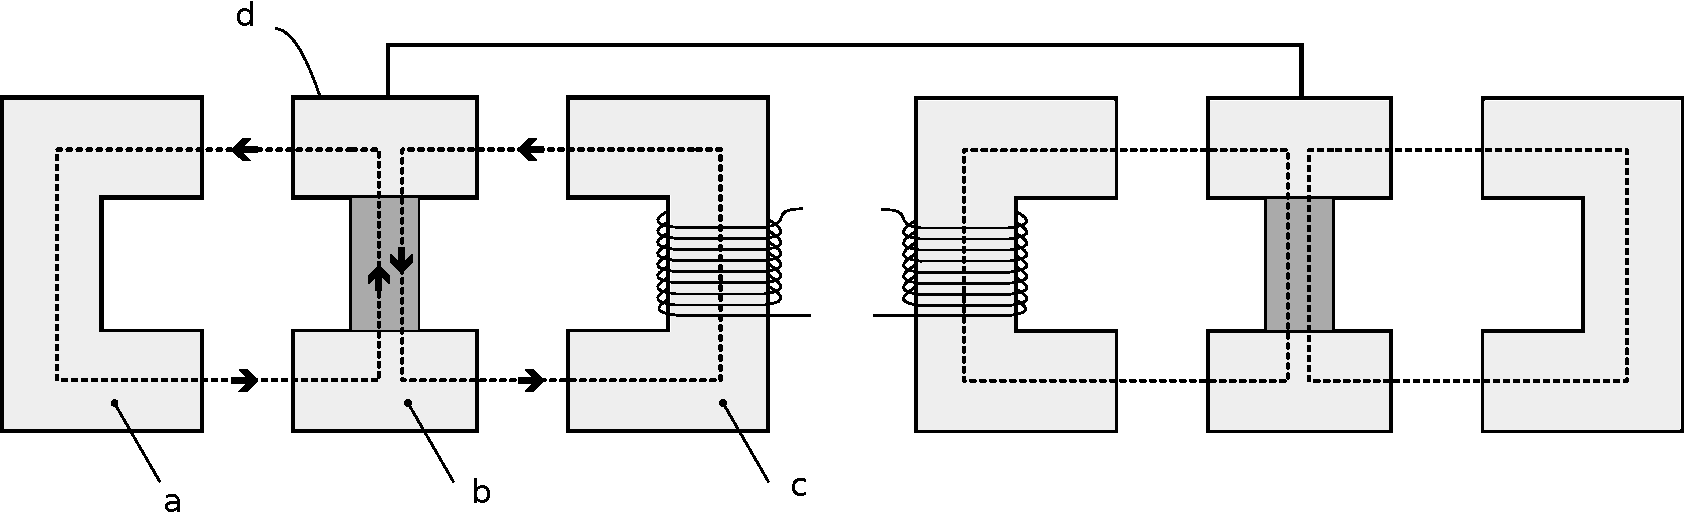
\includegraphics[width=0.7\linewidth]{Figs/mancais/frances}
	\tiny{(1998) Bernus}
	\end{center}
	
	\begin{center}
	\includegraphics[width=0.7\linewidth]{Figs/mancais/alemao}
	\tiny((2001) Scharf)
	\end{center}
	
\end{frame}


\section{O mancal magnético}

\begin{frame}{Mancal magnético}

%\begin{minipage}[c]{0.48\linewidth}
	\begin{itemize}
		\item dois graus de liberdade ativo (radial)
		\item graus de liberdade passivo estabilizados por ímãs permanentes
		\item geometria plana
		\item mancal localizado externo ao motor
		\item escalonável 
	\end{itemize}	
%\end{minipage}
%
%\begin{minipage}[c]{0.46\linewidth}
%	\begin{center}
%	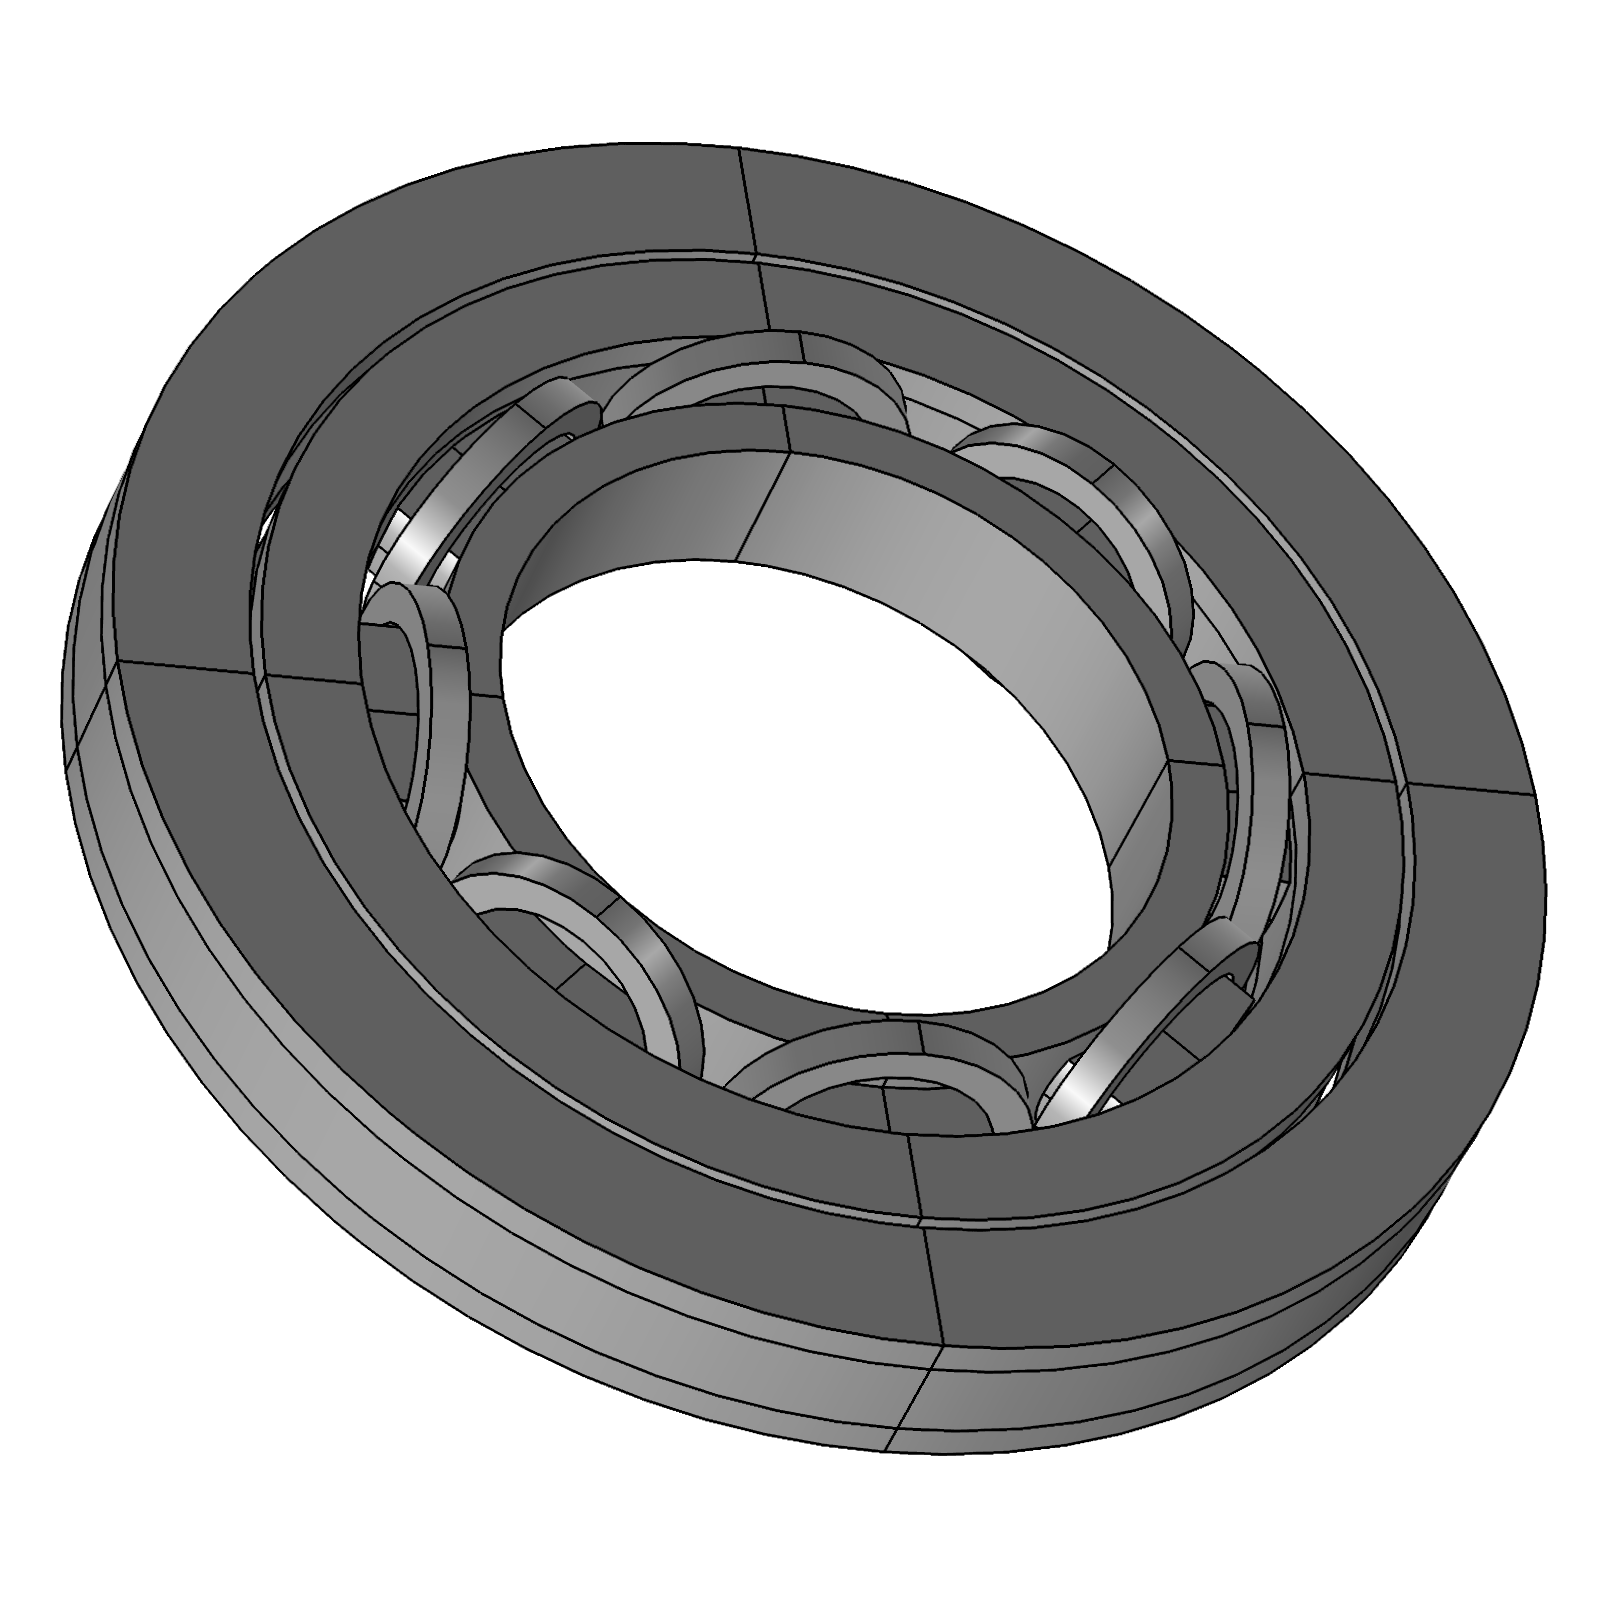
\includegraphics[width=1\linewidth]{Figs/mancais/modelo-elementos-finitos}
%	\end{center}
%\end{minipage}	
\end{frame}

\begin{frame}{Topologia}
\begin{figure}[th!]
\centering
\includegraphics[width=1\linewidth]{Figs/mancais/mancal:corte}

Corte longitudinal do mancal magnético
\label{fig:mancal:corte}
\end{figure}


	\begin{center}
	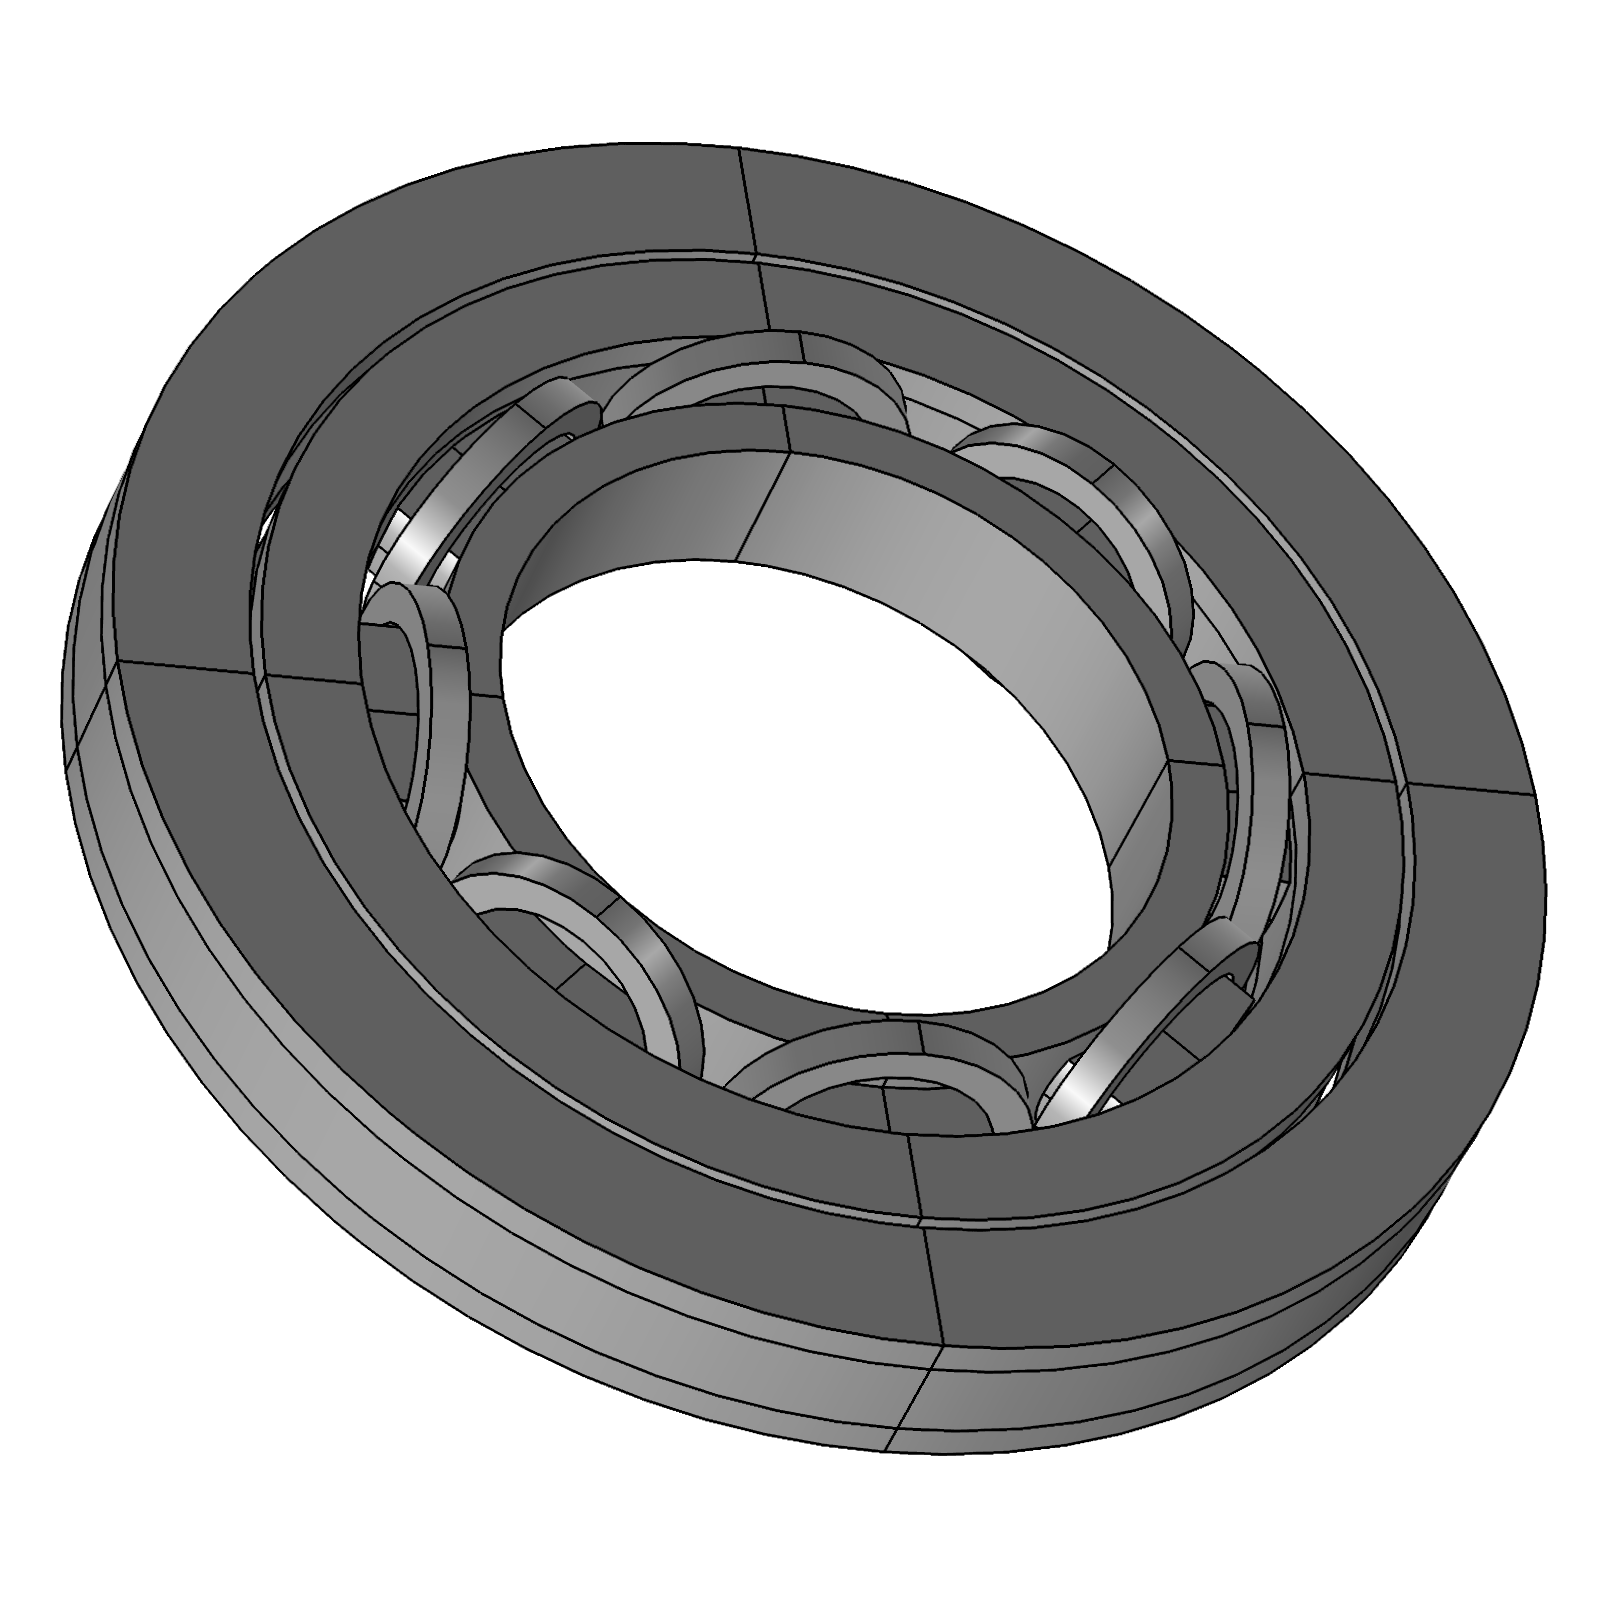
\includegraphics[width=0.4\linewidth]{Figs/mancais/modelo-elementos-finitos}
	\end{center}
\end{frame}


\subsection{Estator Interno}

\begin{frame}{Estator Interno}
	\begin{center}
		\includegraphics[width=0.7\linewidth]{modelo:circuito:passivo:forcas:b}
	\end{center}
\end{frame}	


\begin{frame}{Estator Interno}{Modelagem}
	
\begin{center}
	\includegraphics[width=0.7\linewidth]{circuito:passivo}
\end{center}

	\begin{minipage}[c]{0.48\linewidth}
		\begin{center}
		\includegraphics[width=1\linewidth]{Figs/Simulacoes/Passivo/2D:B:dx=0,6}
		\end{center}
	\end{minipage}
	%
	\begin{minipage}[c]{0.48\linewidth}
		\begin{center}
			\tiny{Força (N) vs Deslocamento radial (mm)}
		\includegraphics[width=1\linewidth]{Figs/Simulacoes/Passivo/forca:passivo:comsol:fx}
		\end{center}
	\end{minipage}	

\end{frame}

\begin{frame}{Estator Interno}{Modelagem/ Força}
	
	\begin{minipage}[c]{0.48\linewidth}
		\begin{center}
		\includegraphics[width=1\linewidth]{Figs/Simulacoes/Passivo/2D:B:dy=1,2}
		\end{center}
	\end{minipage}
	%
	\begin{minipage}[c]{0.48\linewidth}
		\begin{center}
			\tiny{Força (N) vs Deslocamento axial (mm)}
		\includegraphics[width=1\linewidth]{Figs/Simulacoes/Passivo/forca:passivo:comsol:dy}
		\end{center}
	\end{minipage}	

\end{frame}
	
\begin{frame}{Estator Interno}{Modelagem/ Força}

\begin{center}
\includegraphics[width=0.7\linewidth]{Figs/Simulacoes/Passivo/forca:passivo:mod:fx:fy:3d}
\end{center}

\end{frame}


\subsection{Estator Externo}

\begin{frame}{Estator Externo}{}

	\begin{center}
	\includegraphics[width=0.5\linewidth]{Figs/modelo:mancal:estator:interno:fluxo}
	\end{center}
		\begin{center}
		\includegraphics[width=0.5\linewidth]{Figs/modelo:circuito:ativo:explicativo}
		\end{center}
		
\end{frame}

\begin{frame}{Estator Externo}{Modelagem/ Força}

	\begin{minipage}[c]{0.48\linewidth}
		\begin{center}
		\includegraphics[width=1\linewidth]{Figs/Simulacoes/Ativo/comsol:topo:3mm:}
		\end{center}
	\end{minipage}
	%
	\begin{minipage}[c]{0.48\linewidth}
		\begin{center}
		\includegraphics[width=1\linewidth]{Figs/Simulacoes/Ativo/Forca:ativo:comparacao:eq}
		\end{center}
	\end{minipage}	


\end{frame}

\begin{frame}{Batente/ Base}
\begin{center}
\includegraphics[width=0.5\linewidth]{Figs/mancais/mancal:batente:corte}
\end{center}

\end{frame}

\section{Modelo Dinâmico}


\begin{frame}{Modelo dinâmico}{Forças}
\begin{center}
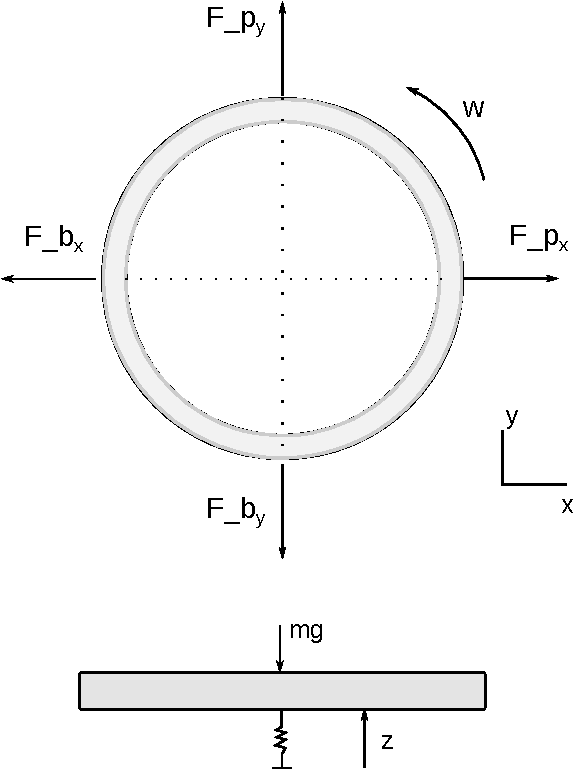
\includegraphics[width=0.5\linewidth]{Figs/Modelagem/forcas}
\end{center}
\end{frame}

\begin{frame}{Modelagem por Lagrange}

   		 \begin{align*}
					T_{\theta, x, y, z} &= \frac{1}{2} I_z \, \dot{\theta}^2 + \frac{1}{2} \, m \, \left( \dot{x}^2 + \dot{y}^2 + \dot{z}^2 \right) \notag \\
				  	V_z &= m \, g \, z + \frac{1}{2} \, K \, z^2\\
				  		L &= T - V \notag  \\
				   		\frac{\partial}{\partial t} \left[ \frac{\partial L}{\partial \dot{r}} \right] -  \frac{\partial L}{\partial r} = Q^{nc} + Q^{c}
   		 \end{align*} 
 
\[\rightarrow\]
   		 \begin{align*}
   			I \ddot{\theta} &= 0 \\
   			m \ddot{x}		&=  F_{px}(x,y) - F_{by}(x,y,i) \\
   			m \ddot{y}		&=  F_{py}(x,y) - F_{bx}(x,y,i)\\	
   			m \ddot{z} - K z &= m g  
   		 \end{align*}
   		
\end{frame}

%\begin{frame}{Batente}{Choque elástico}
%\end{frame}


\begin{frame}{Diagrama de Blocos}

	\begin{center}
	\includegraphics[width=1\linewidth]{Figs/Modelagem/diagrama:blocos:modelo:linear}
	\end{center}
	
	\begin{itemize}
		\item modelo não linear das forças
		\item batente modelado como choque elástico
		\item força contra eletromotriz não modelada 
	\end{itemize}

\end{frame}

\begin{frame}{Modelo Linear }
\[
G_a(s) \, G_p(s) = \frac{46530}{ 0.02077 s^3 + 1.478 s^2 - 3.08e04 s - 2.191e06}
\]
	\begin{center}
	\includegraphics[width=0.7\linewidth]{Figs/Modelagem/bode:rlocus:pnt:operacao}
	\end{center}
\end{frame}

\begin{frame}{Simulações}{Ponto de operação - modelo não linear}
\begin{center}
	\includegraphics[width=0.7\linewidth]{Figs/Modelagem/dinamica:choque:rotor}
\end{center}
\end{frame}

\begin{frame}{Simulações}{Atuador}
\begin{center}
	\includegraphics[width=0.6\linewidth]{Figs/Modelagem/dinamica:corrente:rotor}
\end{center}
\end{frame}

\section{Próximos passos}

\begin{frame}{Problemas}
	\begin{itemize}
		\item usinagem das peças
		\begin{itemize}
			\item ausência de pino guia
			\item tolerância
		\end{itemize}
		\item batente 
		\item embobinamento dos polos
		\item validação do modelo com o protótipo
		\item medida de posição
	\end{itemize}
	
	
	\begin{center}
	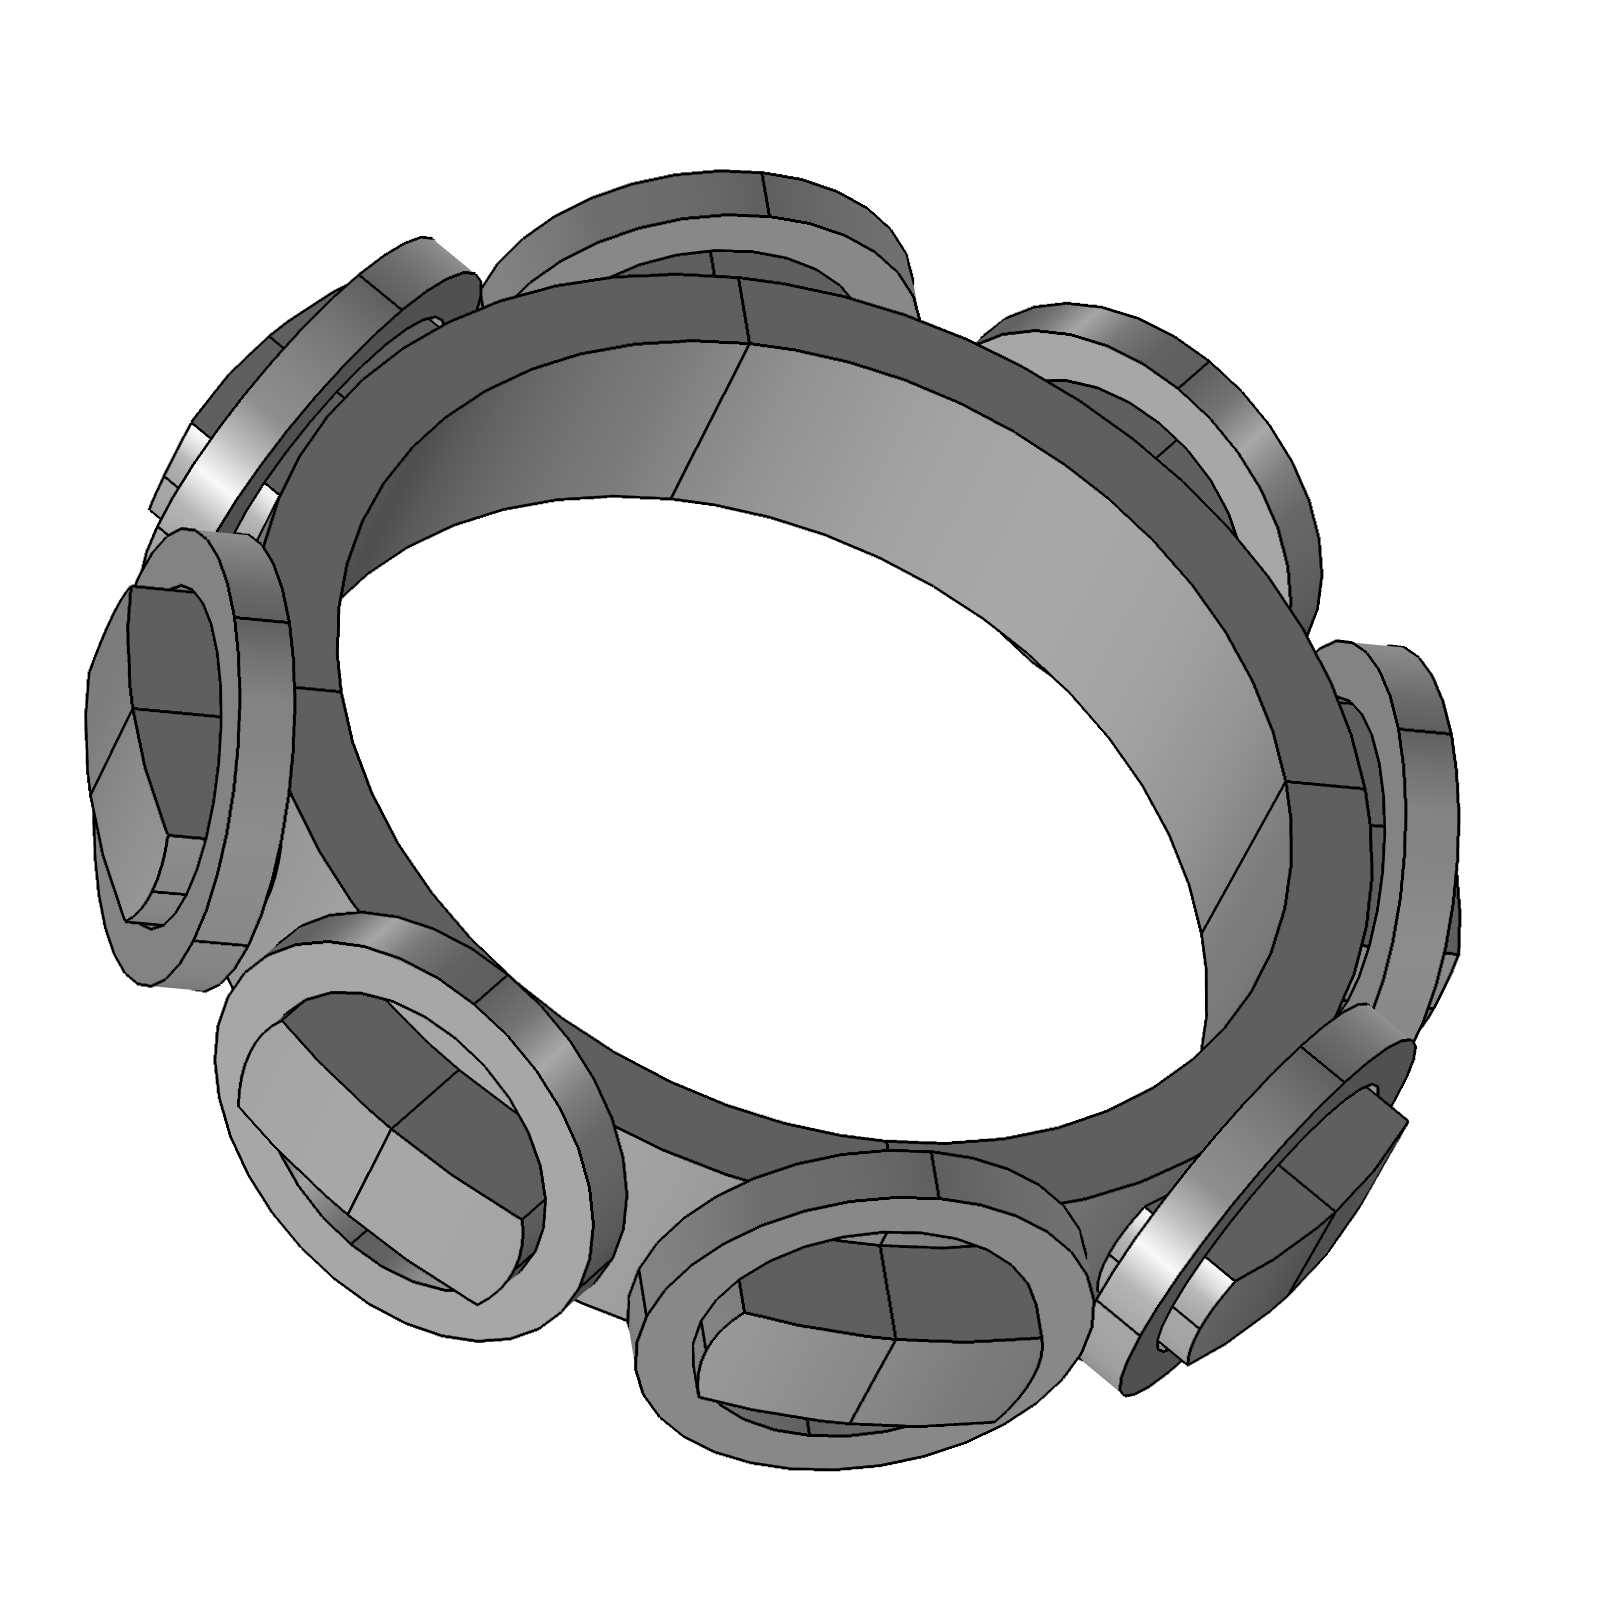
\includegraphics[width=0.3\linewidth]{Figs/mancais/modelo-EI}
	\end{center}
	
\end{frame}

\begin{frame}{Protótipo}
\begin{center}
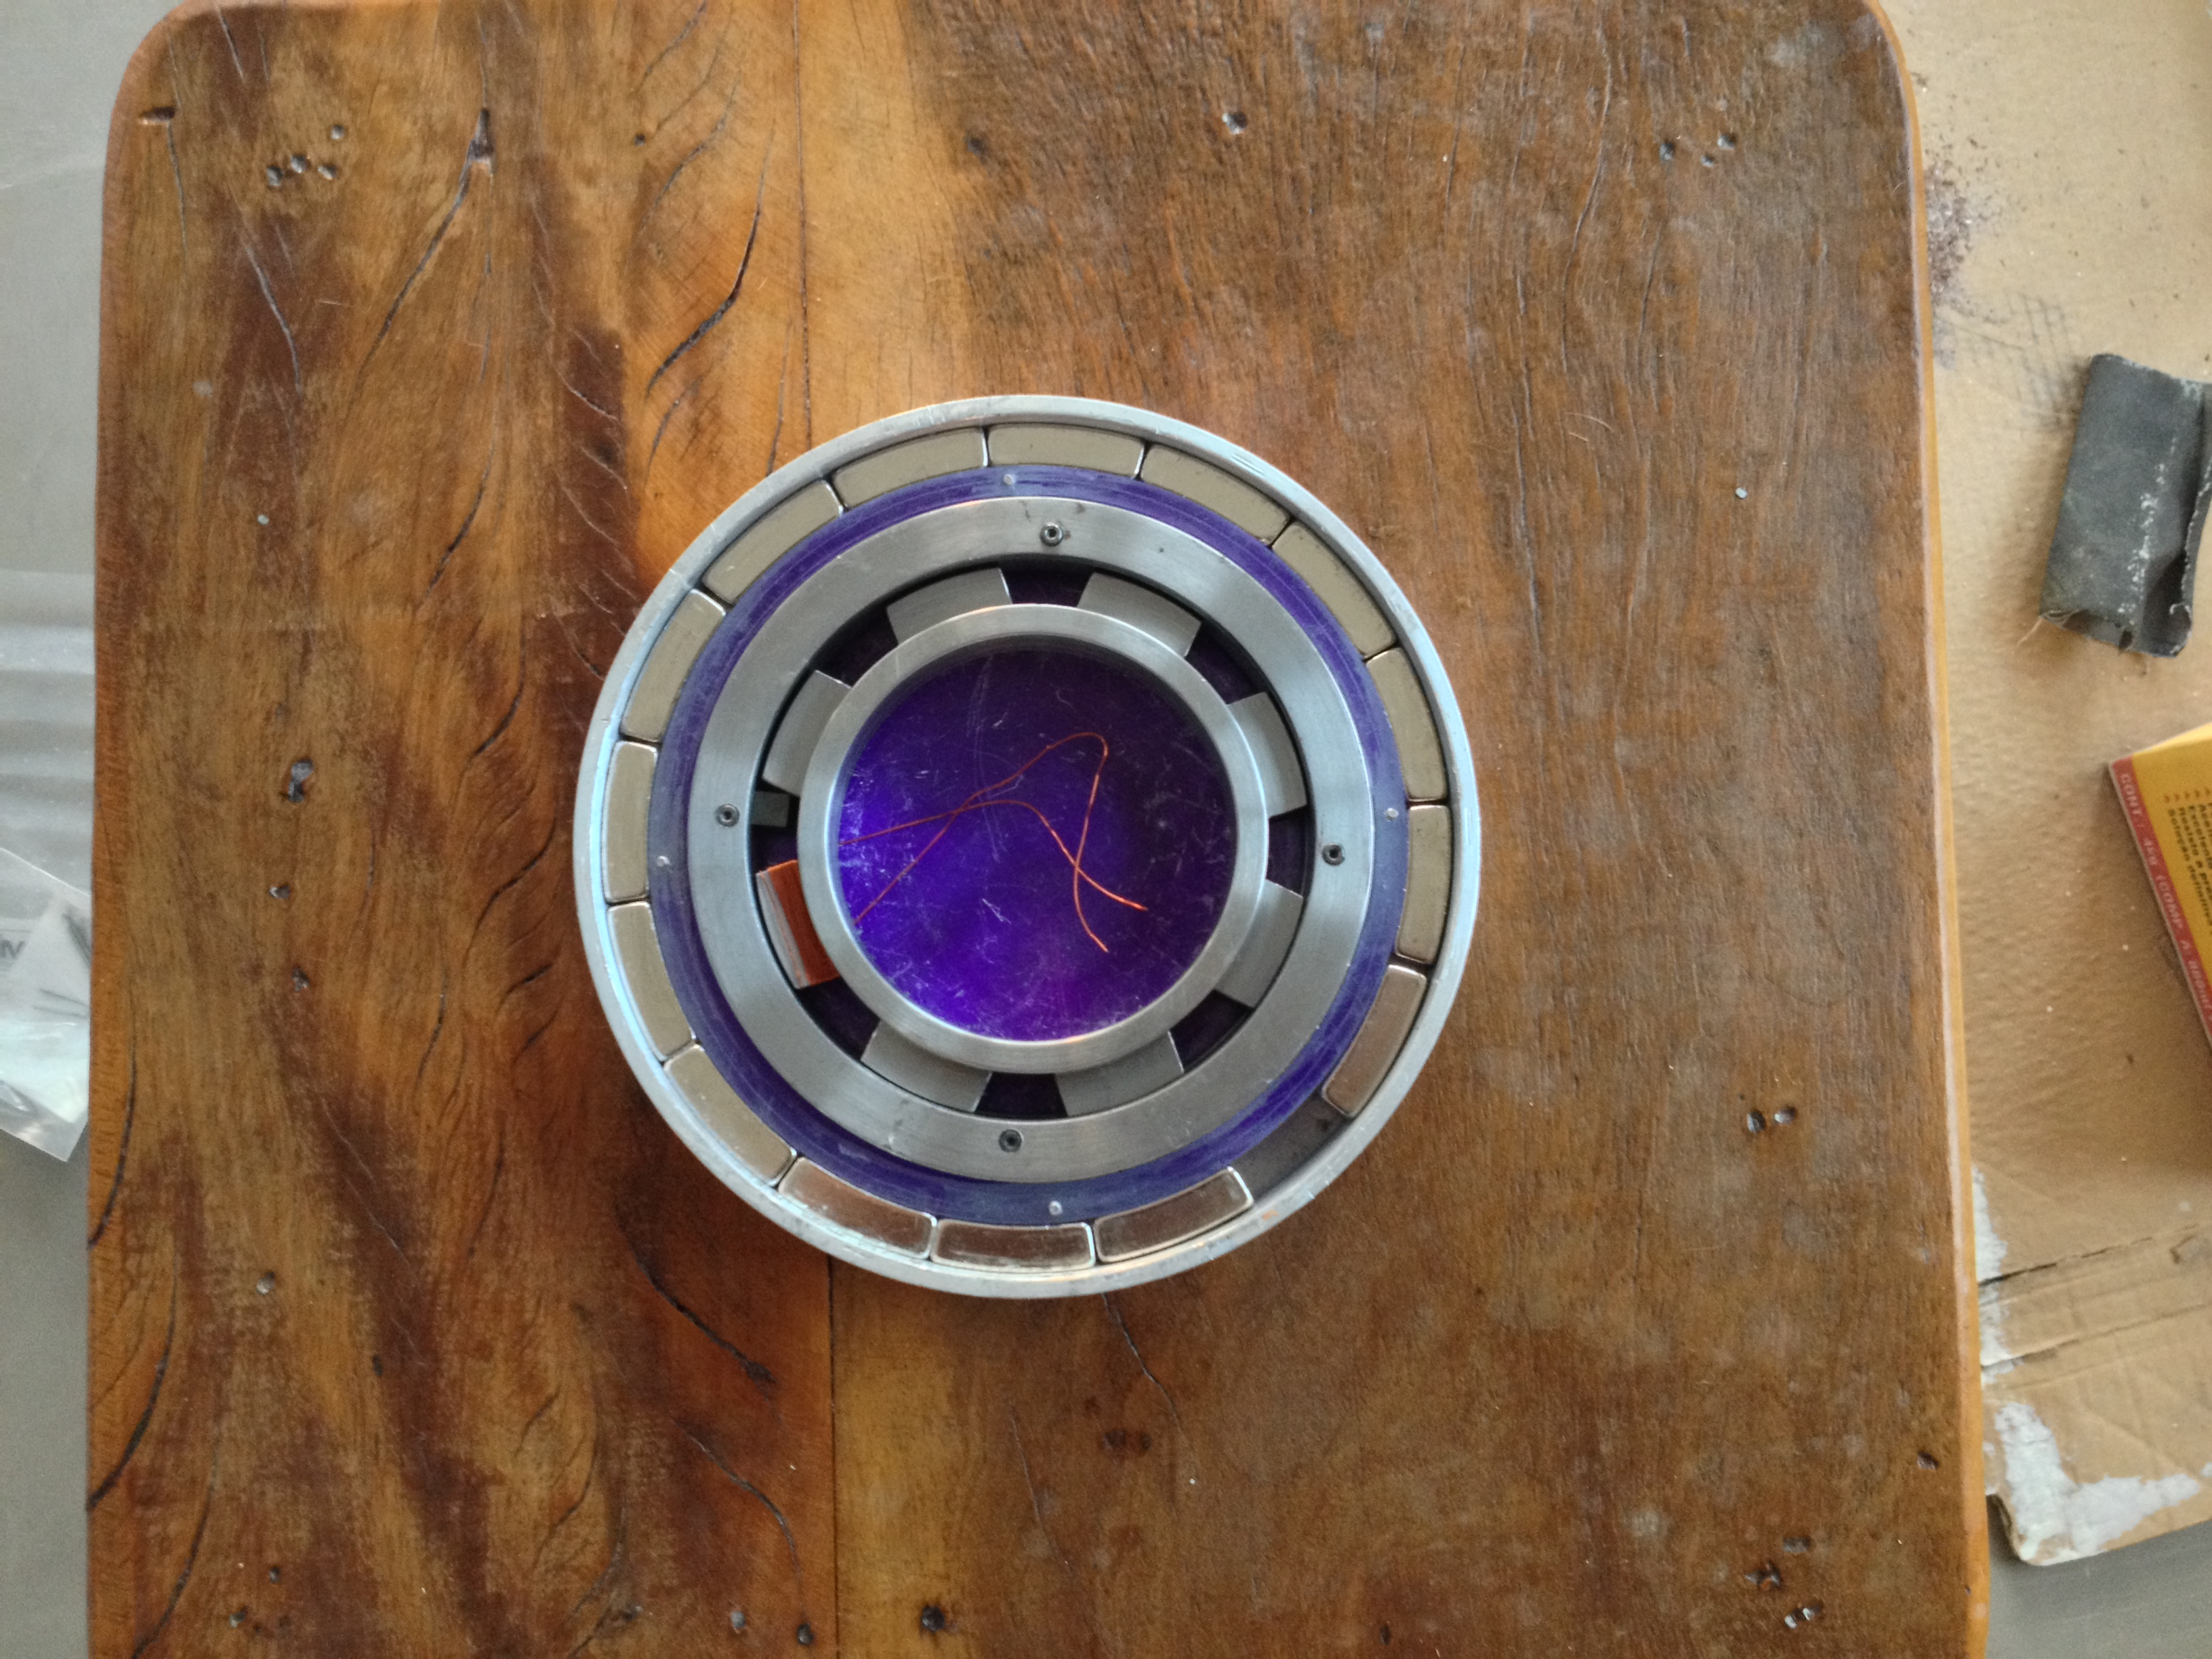
\includegraphics[width=1\linewidth]{2}
\end{center}

\end{frame}

\begin{frame}{Trabalhos Futuros}
\begin{itemize}
	\item correção dos problemas mecânicos
	\item validação do modelo vs protótipo
	\item desenvolvimento do controlador
	\item forma de sensoriamento
	\item desenvolvimento da eletrônica
	\item implementação e testes
\end{itemize}
\end{frame}


% % % % % % % % % % % % % % %
\end{document}
% % % % % % % % % % % % % % %

%\begin{frame} 
%\frametitle{}
%
%\begin{itemize}
%	\item 
%\end{itemize}
%
%\begin{columns}[T] % align columns
%	\begin{column}{.48\textwidth}
%	
%	\end{column}%
%\hfill%
%	\begin{column}{.48\textwidth}
%	
%	\end{column}%
%\end{columns}
%
%\end{frame}
